\author{Troels}
\section{Back--End}
    \subsection{Overview}
        \begin{frame}{Developing the Back--End}\framesubtitle{Overview}
            \begin{itemize}
                \item A REST--API
                \begin{itemize}
                    \item Domain Model Layer
                    \item Persistence Layer
                    \item Service Layer
                    \item 156 Automatic Tests
                \end{itemize}
            \end{itemize}
            \note{We choose to make a REST API ...}
            \note[item]{6 services, 11 endpoints}
        \end{frame}
    \subsection{Technology Stack}
        \begin{frame}{Developing the Back--End}\framesubtitle{Technologies used in the Back--End}
             \begin{itemize}
                 \item Java 8
                 \begin{itemize}
                    \item Spring IoC Container
                    \begin{itemize}
                        \item Inversion of Control
                    \end{itemize}
                    \item Hibernate ORM
                    \begin{itemize}
                        \item Persistence Provider
                    \end{itemize}
                    \item Hibernate Search
                    \begin{itemize}
                        \item Geospatial Queries
                    \end{itemize}
                    \item Flyway
                    \begin{itemize}
                        \item Database Migrations
                    \end{itemize}
                    \item Jackson
                    \begin{itemize}
                        \item JSON (de)serialization 
                    \end{itemize}
                    \item RESTEasy
                    \begin{itemize}
                        \item Mapping Requests to bean methods
                    \end{itemize}
                 \end{itemize}
             \end{itemize}
             \note[item]{Not Java EE (since it's a version behind)}
             \note[item]{Mature technologies in Java}
             \note[item]{Choosen with scalability in mind.}
             \note[item]{Spring BeanFactory Container}
             \note[item]{Spring manages the lifecycle of object and uses dependency injection}
        \end{frame}
        \begin{frame}{Developing the Back--End}\framesubtitle{Technology Stack}
             \begin{figure}
                \pgfdeclarelayer{background}
                \pgfsetlayers{background,main}
                \tikzstyle{bgbox}=[fill=green!20, rounded corners, draw=GoogleGreen, dashed]
                \center
                \begin{tikzpicture}[auto, node distance=1.5cm,
                        stage/.style={rectangle, rounded corners, minimum width=2.5cm, minimum height=1cm,text centered, fill=diagramLight, draw, align=center},
                        sharp/.style={rectangle, minimum width=9.0cm, minimum height=1cm,text centered, fill=diagramLight, draw, align=center},
                        server/.style={rectangle, rounded corners, minimum width=1.5cm, minimum height=1cm,text centered, fill=diagramLight, rectangle split, rectangle split parts=2, draw},
                        flow/.style={draw, ->},
                        reverse_flow/.style={draw, <-},
                        double_flow/.style={draw, <->},
                        create/.style={draw, ->},
                        use/.style={draw, dotted, ->}
                    ]
                    %, line width=0.5mm, draw=black
                    \node (nginx) at (0,0) [stage] {nginx};
                    \node (web2) [draw, cloud, cloud puffs=12, cloud ignores aspect, minimum width=5.5em, minimum height=2.5em,fill=blue!20, above=0.6cm of nginx] {Internet};

                    
                    \node (wildfly) [stage, minimum height=2.2cm, below=0.6cm of nginx] {};
                    \node [below=0.1cm] at (wildfly.north) {Wildfly};
                    \node (ourcode) [stage, above=0.2cm, fill=GoogleGreen, minimum width=2.0cm] at (wildfly.south) {Our Code};

                    \node (lucene) [stage, below left=0.6cm of wildfly] {Lucene};
                    \node (postgres) [stage, below right=0.6cm of wildfly] {PostgreSQL};

                    \draw [double_flow] (nginx) -- (web2);
                    \draw [double_flow] (nginx) -- (wildfly);
                    \draw [double_flow] (wildfly) -| (postgres);
                    \draw [double_flow] (ourcode.west) -| (lucene);
                \end{tikzpicture}
            \end{figure}
            \note[item]{Our system is more parts!}
            \note[item]{Previously we used MongoDB instead of PostgreSQL}
        \end{frame}

    \subsection{Data}
        \begin{frame}[t]{Developing the Back--End}\framesubtitle{The Model}
            \only<1|handout:1> {
            \begin{figure}[htb]
                \centering
                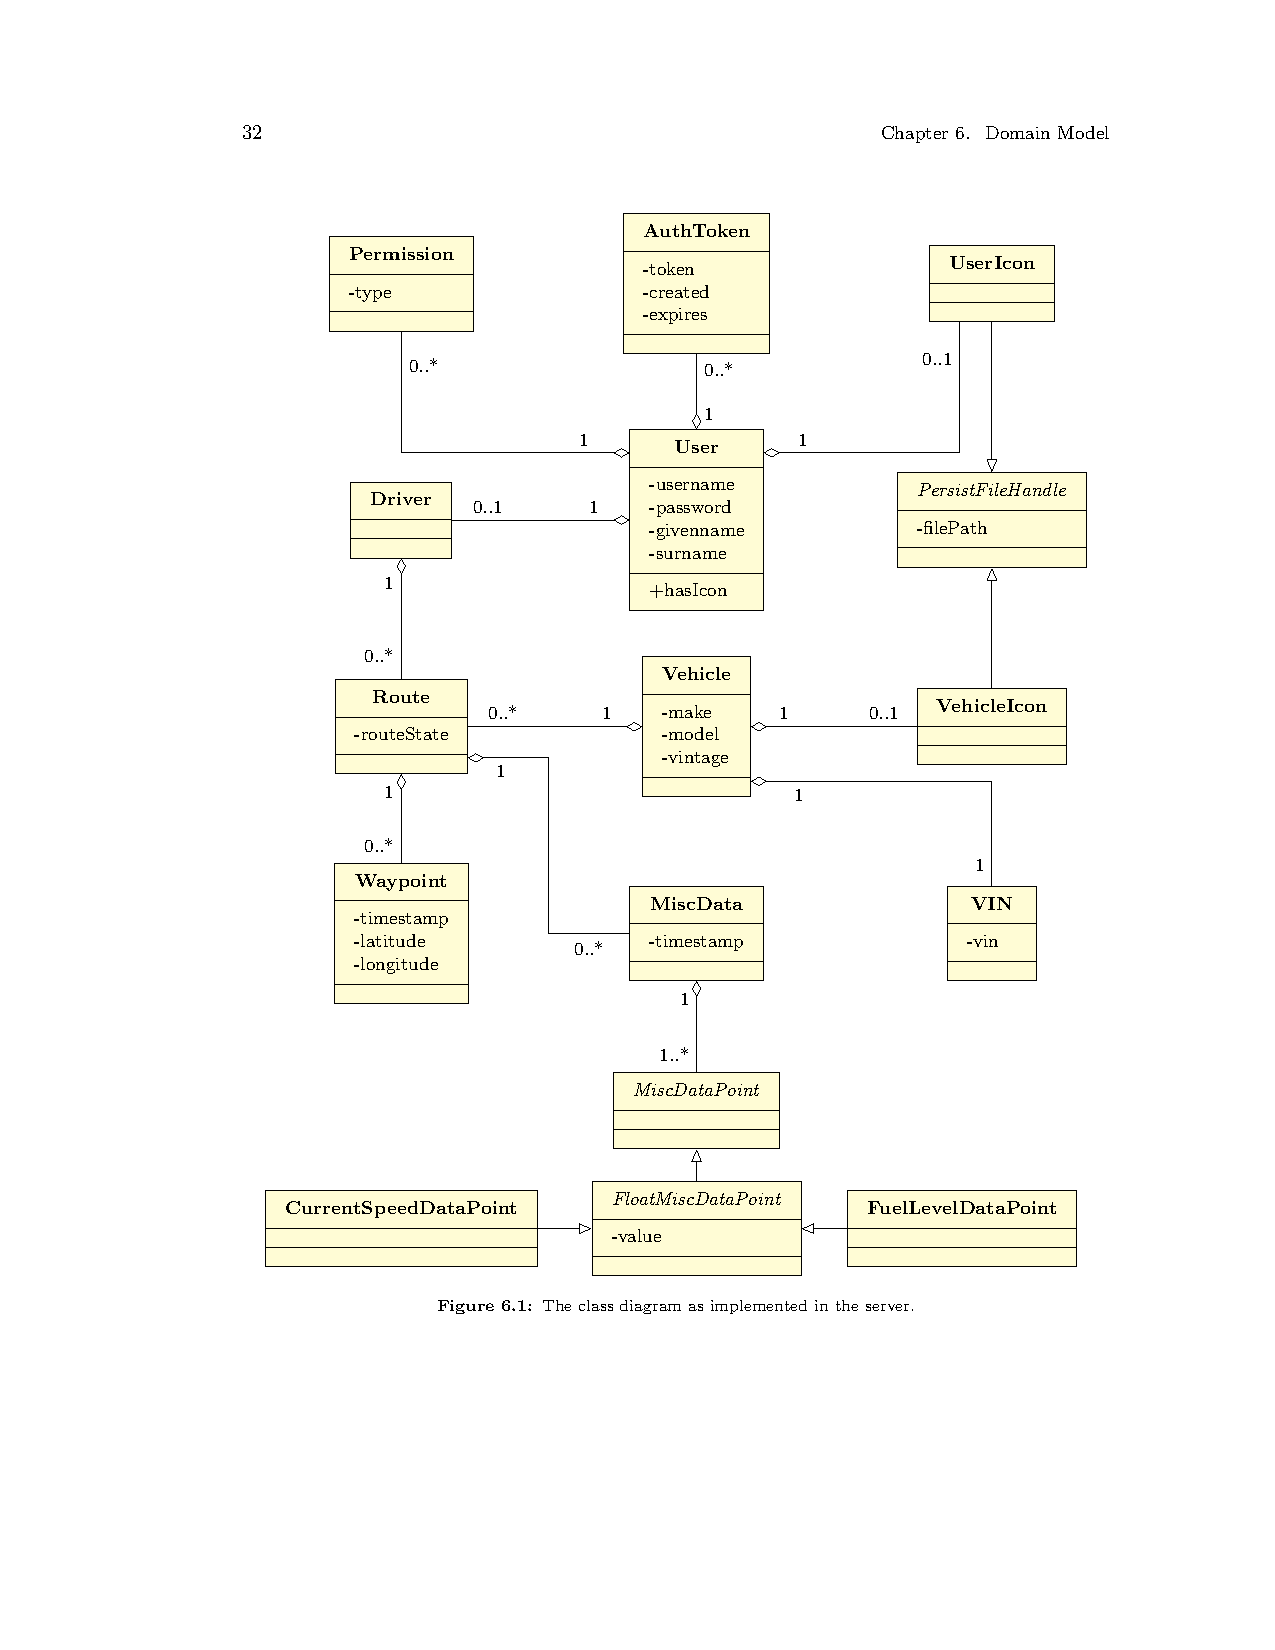
\includegraphics[width=0.60\textwidth, trim={4.2cm 6.0cm 2.5cm 3.5cm},clip]{class.pdf}
            \end{figure}
            \note<1>[item]{Designed with expandability in mind}
            \note<1>[item]{Driver as ``has a''}
            \note<1>[item]{MiscData on Route}
            }

            \only<2|handout:2> {
            Driver as ``has a'':
            \begin{figure}[htb]
                \centering
                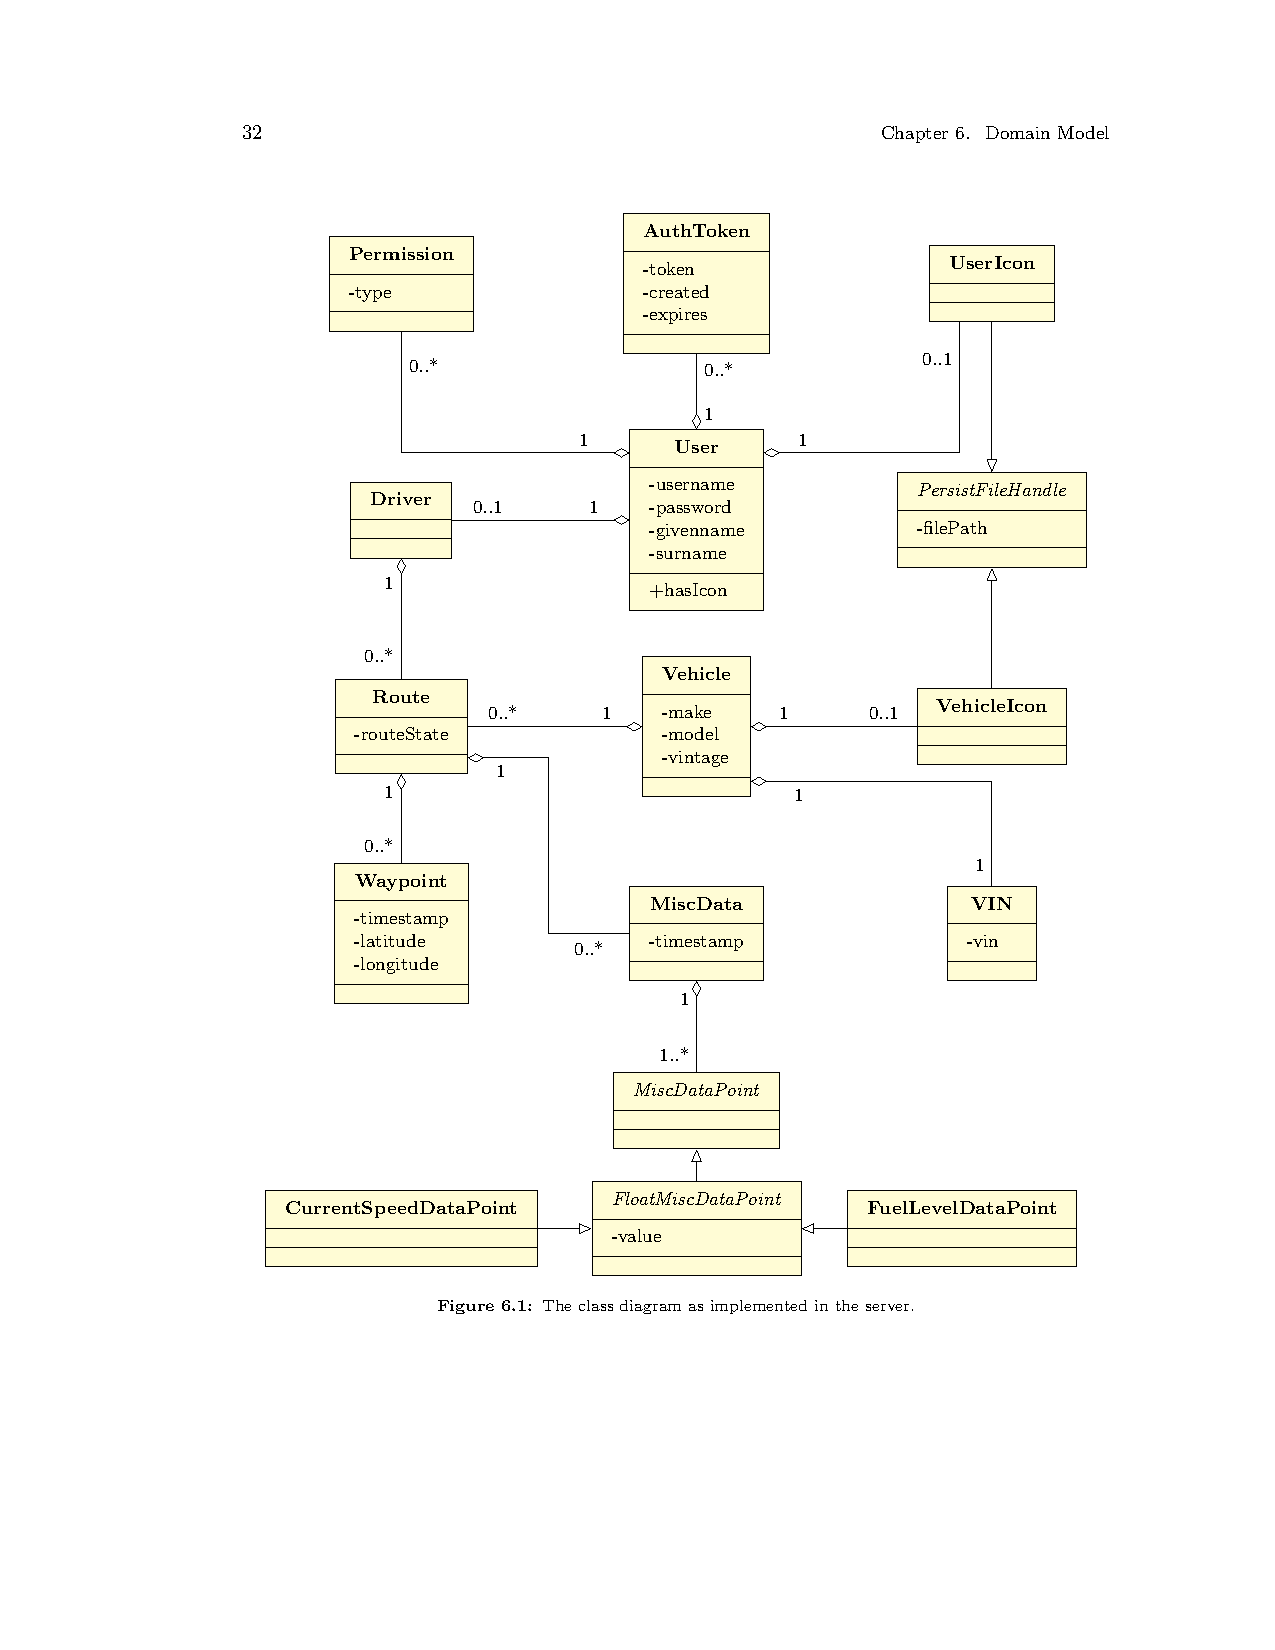
\includegraphics[width=0.85\textwidth, trim={5cm 13.8cm 0cm 3.5cm},clip]{class.pdf}
            \end{figure}
            \note<2>[item]{Expandability to other ``roles'' than driver, i.e. manager}
            \note<2>[item]{Role pattern (is-a)}
            }

            \only<3|handout:3> {
            MiscData on Route:
            \begin{figure}[htb]
                \centering
                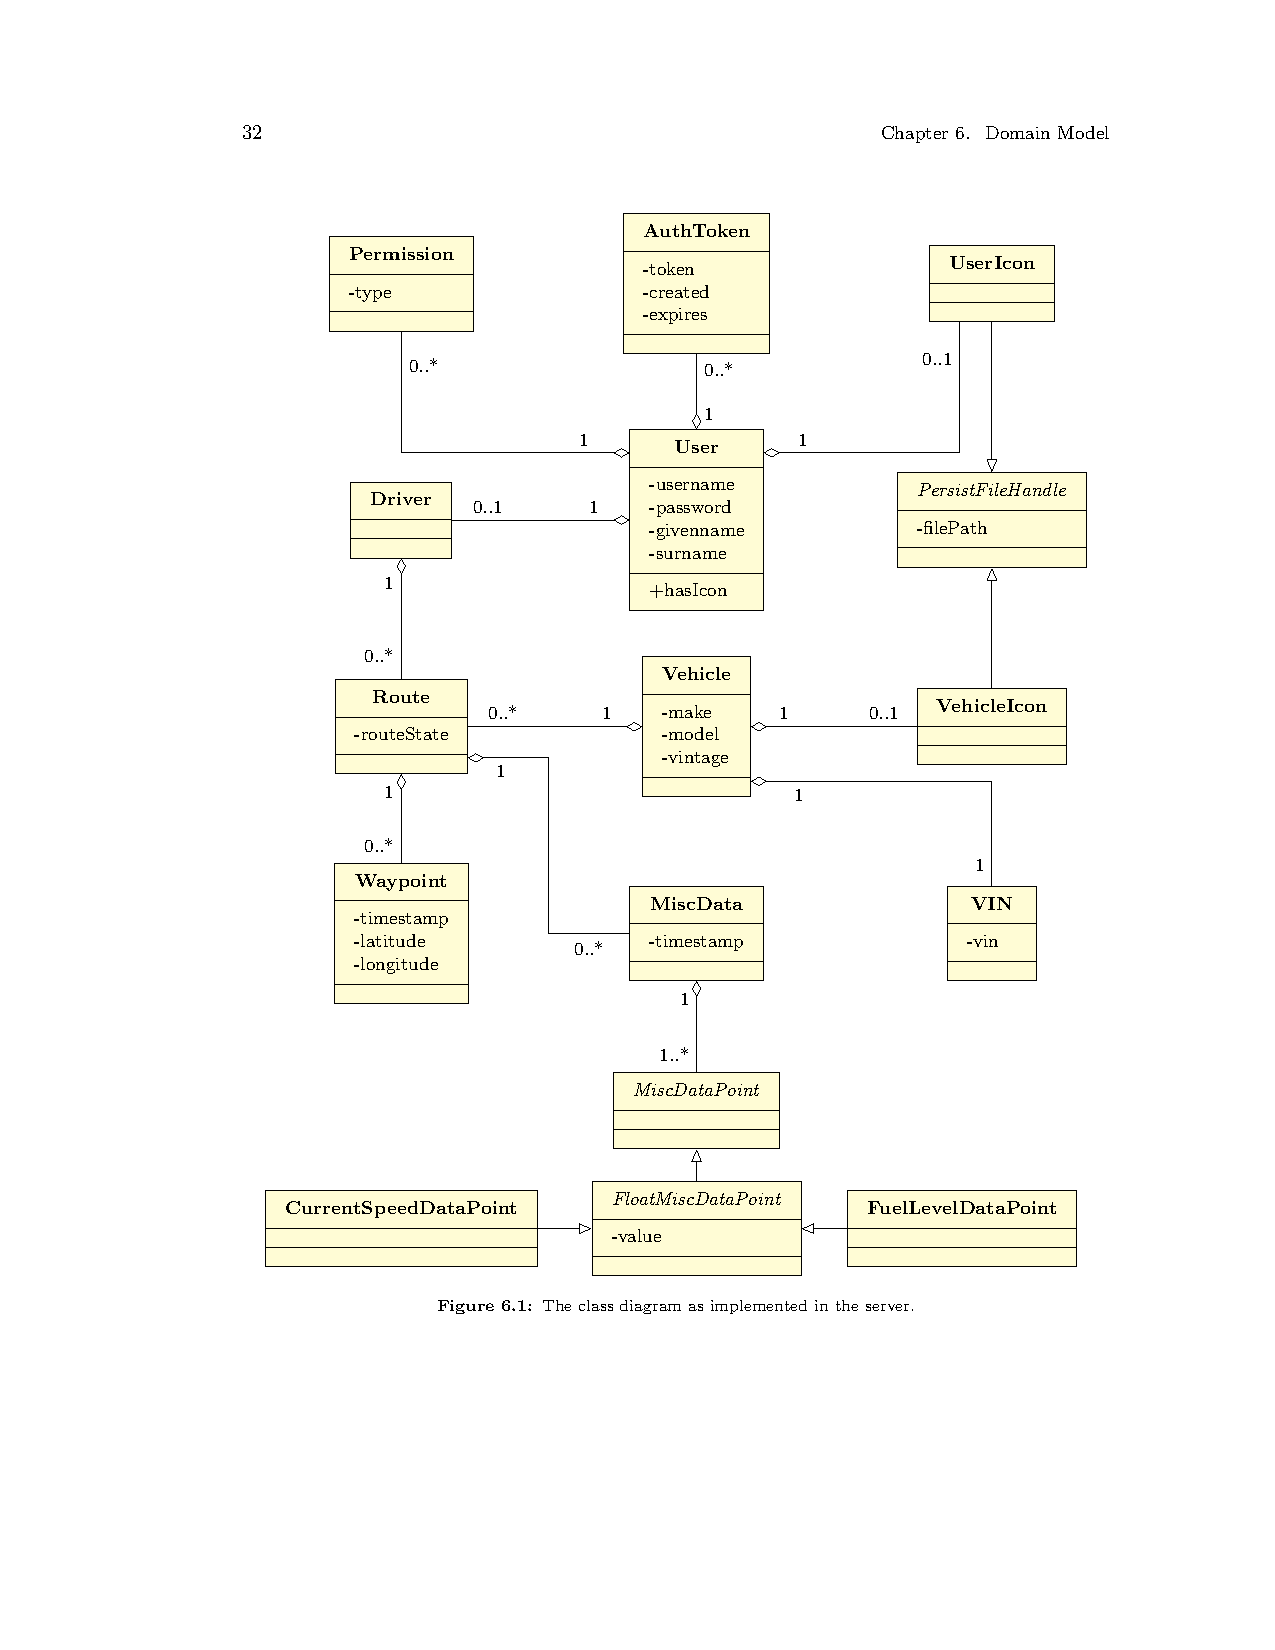
\includegraphics[width=0.85\textwidth, trim={4.2cm 6.0cm 2.5cm 11cm},clip]{class.pdf}
            \end{figure}
            \note<3>[item]{MiscData indirectly to vehicle currently}
            \note<3>[item]{Context of use.}
            \note<3>[item]{MiscData <-> Maintence <-> Vehicle}
            \note<3>[item]{Maintence: Vehicle, Time, details, cost etc. AND MiscData}
            }
        \end{frame}

    \subsection{Endpoints}
        \begin{frame}{Developing the Back--End}\framesubtitle{API Endpoints}
            \begin{table}[ht]
                \centering
                \scriptsize
                \begin{tabu} to \textwidth {llXl}
                    HTTP Methods       & Endpoint               & Service     \\ \midrule
                    \texttt{GET}, \texttt{POST} & /auth                    & \texttt{AuthService}\\ \tblgrpsep
                    \texttt{GET}, \texttt{POST} & /user                    & \multirow{3}{*}{\texttt{UserService}}\\
                    \texttt{GET}, \texttt{PUT}  & /user/\{uid\}            & \\
                    \texttt{GET}, \texttt{PUT}  & /user/\{uid\}/icon       & \\ \tblgrpsep
                    \texttt{GET}, \texttt{POST} & /vehicle                 & \multirow{3}{*}{\texttt{VehicleService}}\\
                    \texttt{GET}, \texttt{PUT}  & /vehicle/\{vid\}         & \\
                    \texttt{GET}, \texttt{PUT}  & /vehicle/\{vid\}/icon    & \\ \tblgrpsep
                    \texttt{GET}, \texttt{POST} & /route                   & \multirow{2}{*}{\texttt{RouteService}}\\
                    \texttt{GET}, \texttt{PUT}  & /route/\{rid\}           & \\
                    \texttt{GET}, \texttt{POST} & /route/\{rid\}/waypoint  & \texttt{WaypointService}\\
                    \texttt{GET}, \texttt{POST} & /route/\{rid\}/datapoint & \texttt{MiscDataService}\\
                \end{tabu}
                \caption{A table corrolating the endpoints and services.}\label{table:endpointservice}
            \end{table}
            \note<1>[item]{11 endpoints}
            \note<1>[item]{Seperated into services}
            \note<1>[item]{No deletion}
            
        \end{frame}

    \subsection{Example of use}
        \begin{frame}{Developing the Back--End}\framesubtitle{Adding a new waypoint}
            Endpoint: \texttt{POST /route/100/waypoint} 
            \\
            Request:
            \jsoncode{slides/restapi/req1.json}
            \bigskip
            Response:
            \jsoncode{slides/restapi/res1.json}
            \note[item]{Creating an object returns the object created.}
        \end{frame}

        \begin{frame}{Developing the Back--End}\framesubtitle{A Spatial Query}
            Endpoint: \texttt{GET /route?latitude=56.0\&longitude=10.0\&radius=10}
            \\
            Response:
            \jsoncode{slides/restapi/res2.json}
            \note[item]{Query parameter}
            \note[item]{Works by finding waypoints, and returns their routes.}
            \note[item]{Pagination}
        \end{frame}
